\clearpage{\pagestyle{empty}\cleardoublepage}
\chapter{Applicazioni di schiumogeno per l'ottimizzazione della produzione degli idrocarburi}
\chaptermark{Applicazioni di schiumogeno}
\
\section{Introduzione}
Per \textit{Gas Well Deliquification} o \textit{Gas Well Dewatering} si intende l'insieme delle tecnologie e delle applciazioni utili alla rimozione di acqua o condensati in fase produttiva da un pozzo a gas. Nello specifico il concetto di GDW racchiude tutti gli strumenti utili nel combattere il fenomeno del \textit{liquid loading}, definito come l'impossibilità di un pozzo a gas di rimuovere liquidi prodotti in pozzo. 

\section{Liquid loading}
\subsection{Ciclo di vita di un pozzo a gas}
Nel paragrafo \ref{sssec:verticali} si è discusso dei diversi tipi regimi di flusso bifase per condotte verticali. Un pozzo a gas può presentare tutti i regimi di flusso: in \figref{fig:wellhistory} è possibile comprendere graficamente l'evoluzione del pozzo durante il suo ciclo di vita.

\begin{figure}[htbp]
    \centering
    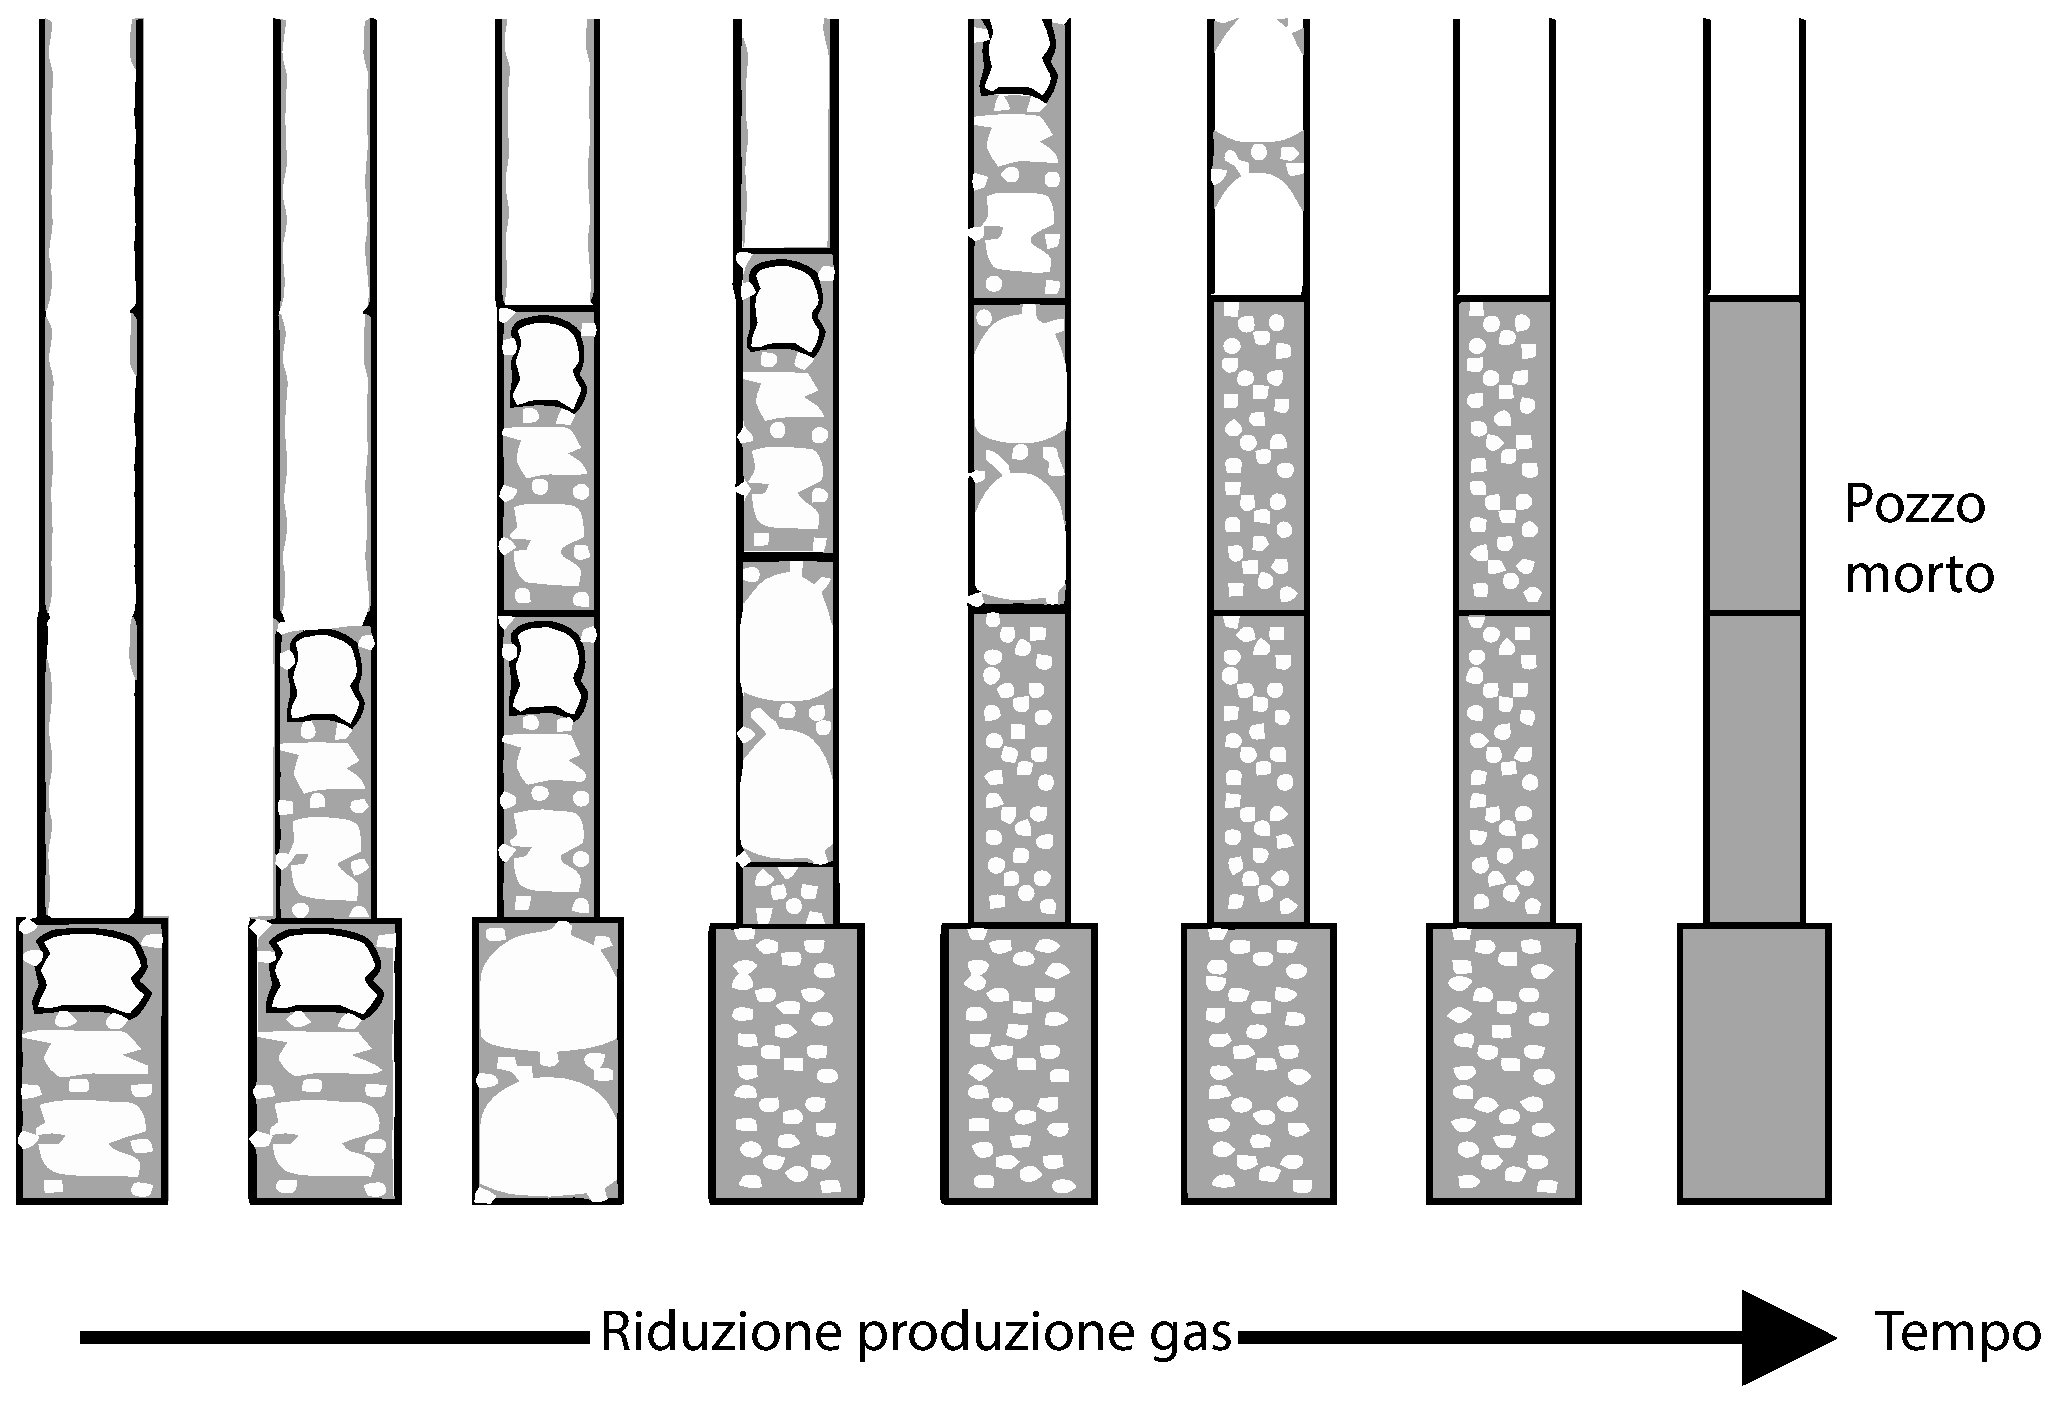
\includegraphics[width=.8\textwidth]{fig/foamer/wellhistory.eps}
    \caption{Schematizzazione del ciclo di vita di un pozzo a gas}
    \label{fig:wellhistory}
\end{figure}

Generalmente in un pozzo sono presenti tutti i diversi regimi di flusso, con il passare del tempo varia la distribuzione dei diversi pattern lungo il tubino di produzione. Inizialmente il gas è fase dominante nel pozzo e ha forza sufficiente per trascinare tutto il liquido presente fondo pozzo. Ad alte velocità superficiali del gas corrisponde un regime anulare misto: la fase liquida è interdispersa nella fase gassosa. Con il diminuire della velocità del gas nel tempo, la fase liquida comincia a precipitare e a depositarsi sul fondo, ostacolando la normale produzione di gas.

\subsection{Problemi legati al liquid loading}
Il liquid loading porta a un regime di flusso a slug e a una produzione di gas discontinua e inferiore. Se il gas ha energia sufficiente a rimuovere i liquidi presenti a fondo pozzo, la portata del gas risponde in modo corretto alla stima di produzione rispetto al tempo di vita del pozzo, definita per via grafica dalla \textit{Decline Curve Analysis} (DAC).

CORREGGERE IMMAGINE, INTRODURRE IN ORDINATA PORTATA
\begin{figure}[htbp]
    \centering
    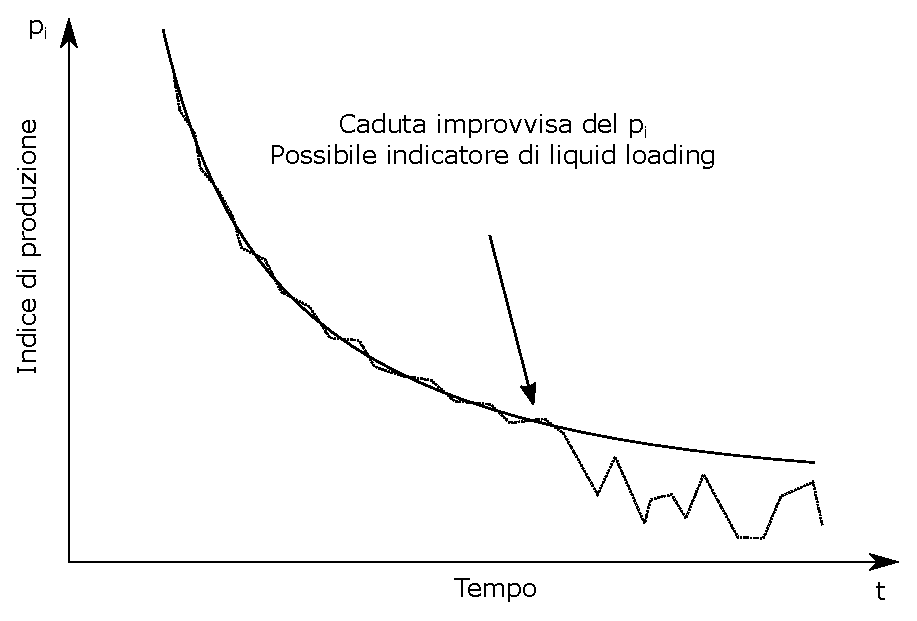
\includegraphics[width=.8\textwidth]{fig/foamer/declinecurve.eps}
    \caption{Analisi della curva di declino.}
    \label{fig:ipr}
\end{figure}

In caso di aumento della colonna idrostatica, il pozzo produce gas in quantità minore rispetto alle stime effettuate. Raggiunto uno stato critico di produzione di gas, il giacimento non ha più energia sufficiente per lo spiazzamento del pozzo e l'effetto combinato di precipitazione di liquidi a fondo pozzo e diminuzione fisiologica della pressione di giacimento porta all'innalzamento della colonna idrostatica. L'aumento dell'altezza della colonna di liquido può quindi terminare la produzione, sancendo così il termine del ciclo di vita del pozzo stesso.
 
\subsection{Sorgenti di liquidi per un pozzo a gas}
Nella maggior parte dei pozzi la produzione di gas è associata a produzione di liquidi. Questi liquidi possono essere acqua, vapore acqueo condensato o idrocarburi condensati. I liquidi prodotti in pozzo dipendono dalle condizioni e dal tipo di giacimento in questione. Le principali cause possono essere:

\begin{itemize}
    \item \textbf{\textit{water coning}}: in un giacimento caratterizato da una falda a gas collocata su una falda d'acqua, alti valori di produzione di gas corrispondono a una repentina caduta di pressione locale; la superficie di separazione delle due fasi assume la configurazione di un conoide e la fase liquida invade così la perforazione;
    \item \textbf{acqua da acquifero}: se la coltivazione del giacimento avviene per mezzo della spinta dell'acquifero (\textit{water-drive}) l'acqua può viaggiare fino a raggiungere la perforazione;
    \item \textbf{vapore acqueo condensato}: poiché nei giacimenti è pressoché sempre presente acqua di strato, il gas naturale è associato a vapore acqueo che, se le condizioni di pressione e temperatura sono tali da scendere al di sotto del punto di rugiada, condensa e contribuisce al quantitativo totale di acqua di produzione;
    \item \textbf{idrocarburi condensati}: come il vapore acqueo, alcuni idrocarburi pregiati possono passare dallo stato gassoso allo stato liquido con il variare delle condizioni di pressione e temperatura;
    \item \textbf{acqua di produzione da un'altra zona}: specialmente nelle operazioni di completamento a foro aperto o in alcuni casi di perforazioni multiple, è possibile che dei liquidi possano confluire nel pozzo tramite vie preferenziali (fratturazioni dell'ammasso roccioso);
    \item \textbf{acqua di formazione}: l'acqua può essere prodotta assieme al gas dalla stessa perforazione se è presente acqua libera di formazione.
\end{itemize}

\subsection{Velocità critica}
La velocità terminale è definita come la velocità di caduta di un corpo libero (la precipitazione particelle liquide) in un mezzo fluido (il gas naturale) sotto l'influenza della forza di gravità. La \textit{velocità critica} è basata sulla velocità terminale delle particelle di liquido, aumentata però di una quantità finita per garantire lo spiazzamento del liquido dal pozzo. Il primo a creare un modello sperimentale inerente al trascinamento continuo di liquido fu \textcite{turner1969analysis}. L'equazione teorica per la velocità critica \(w_t\) per il trascinamento verticale di una goccia:
\[w_t= 1,593\dfrac{\sigma{(\rho_l-\rho_g)}}{\rho_g^2}^{1/4} \qquad\textrm{[ft/sec]} \addtag \label{eq:turnerwc} \]
Poiché in campo le condizioni variano molto rispetto al modello teorico, l'autore fornisce due equazioni relative al trascinamento di acqua (\(w_{c,w}\)) o condensati (\(w_{c,cond}\)):
\[w_{c,w} = 5,304 \dfrac{(67-0,0031p)^{1/4}}{\sqrt{0,0031p}}  \qquad\textrm{[ft/sec]} \label{eq:w_c,w} \addtag\]
\[w_{c,cond} = 4,03 \dfrac{(45-0,0031p)^{1/4}}{\sqrt{0,0031p}}  \qquad\textrm{[ft/sec]} \label{eq:w_c,cond} \addtag\]
Dalla \eqref{eq:w_c,w} e la \eqref{eq:w_c,cond} si ricava il valore della portata critica giornaliera:
\[Q_{c,giorno}=\dfrac{3,06 \; w_c \; p \; A}{T \; Z}  \qquad \textrm{[MMft\ap{3}/giorno]} \addtag \]
dove \(w_c\) fa riferimento o alla velocità critica per acqua o condensati. Tutte i parametri e le variabili del modello sono espressi nel sistema consuetudinario statunitense. \\
Negli anni successivi la ricerca ha portato alla creazione di ulteriori modelli sempre più raffinati: \textcite{coleman1991new} utilizza il modello di \citeauthor{turner1969analysis} ma lo convalida per pressioni di testa pozzo sopra i 35 bar, \textcite{li2001new} crea un modello basato sulla forma appiattita delle particelle liquide, \textcite{nosseir1997new} formula un modello che si adatta alle condizioni di flusso.

\subsection{Analisi nodale}
La velocità critica è impiegata nell'analisi nodale, al fine di verificare che le condizioni di produzione ottimali consentano anche il trascinamento dell'acqua da fondo pozzo.\\
L'analisi nodale divide il sistema in due sottosistemi:
\begin{itemize}
    \item \textbf{\textit{Inflow Production Relationship} (IPR)}: valuta il valore della portata in funzione della pressione a fondo pozzo;
    \item \textbf{\textit{Tubing Performance Relationship} (TPR) o \textit{Vertical Lift Performance} (VLP)}: mostra il rapporto tra le cadute di pressione in pozzo e la portata, nasce dalla combinazione delle cadute di pressione (sempre in funzione della produzione) per effetto della gravità del flusso e dell'attrito della condotta.
\end{itemize}
La produttività del pozzo si ottiene dall'intersezione dell'IPR con la TPR. Il punto trovato viene definito \textit{punto operativo ottimale}, dove i valori di pressione e produttività sono uguali in ambo le curve. Se si traccia sullo stesso grafico il valore di velocità critica (\figref{fig:ipr-tpr}), quindi di portata critica, si può stabilire se le condizioni operative ottimali impediscono la precipitazione della fase liquidi a fondo pozzo. Se il punto di intersezione tra l'IPR e la TPR si trova a destra della curva relativa alla velocità critica, il pozzo ha energia sufficiente per trascinare interamente la fase liquida, altrimenti si incorre nel fenomeno di liquid loading.

\begin{figure}[htbp]
    \centering
    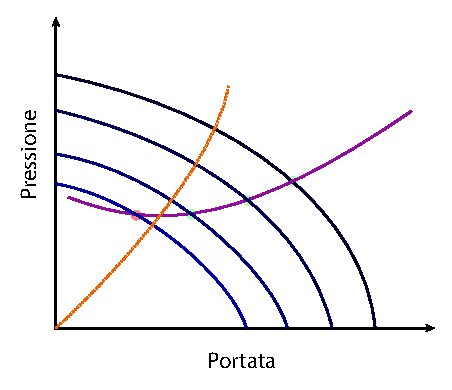
\includegraphics[width=.5\textwidth]{fig/foamer/ipr-tpr.eps}
    \caption{Analisi nodale combinata alla portata critica di trascinamento}
    \label{fig:ipr-tpr}
\end{figure}


\section[Artificial lift per GDW]{Sistemi di sollevamento artificiale per il Gas Well Deliquification}
\sectionmark{Artificial lift per GDW}
L'industria del gas utilizza numerosi metodi per la rimozione di liquidi dai pozzi. Qui di seguito sono presentati i metodi più utilizzati e ormai consolidati nel tempo con particolare attenzione agli schiumogeni a cui è dedicata una sezione a parte. \textcite{oyewole2008artificial} classifica i sistemi di sollevamento artificiale in:
\begin{itemize}
    \item \textbf{a energia del giacimento}: qui definiti  \textit{a energia interna}, i sistemi non aumentano direttamente l'energia del giacimento, bensì agiscono sui parametri che caratterizzano il trascinamento del liquido in pozzo;
    \item \textbf{a energia esterna}: sistemi a fondo pozzo che agiscono indipendentemente dall'energia residua del giacimento.
\end{itemize}
Le velocity string, i compressori, i plunger e gli schiumogeni sono sistemi di sollevamento artificiale a energia interna, pompe e iniezione di fluidi sono invece sistemi \textit{a energia esterna}.

\subsection{Velocity string}
La velocity string è praticamente un tubino di produzione con diametro inferiore rispetto a quello già presente in situ. Per produzione costante, il restringimento della sezione di produzione provoca un aumento della velocità del flusso in condotta e il superamento del valore della velocità critica. L'applicazione può avvenire su un tratto specifico del pozzo (\figref{fig:velocitystring-fixed}) oppure su tutta la lunghezza del pozzo (\figref{fig:velocitystring-long}).

\begin{figure}[htbp]
\centering
    \subfloat[][Lunghezza fissa]
    {\makebox[0.4\textwidth]{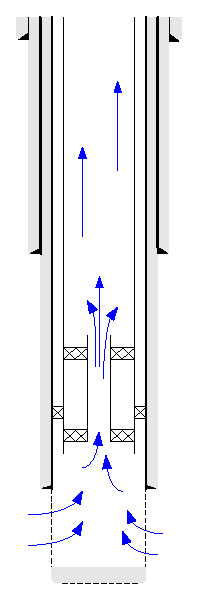
\includegraphics[width=.15\textwidth]{fig/foamer/velocitystring/velocitystring-fixed.eps}} \label{fig:velocitystring-fixed}} \quad
    \subfloat[][Su tutto il pozzo]
    {\makebox[0.4\textwidth]{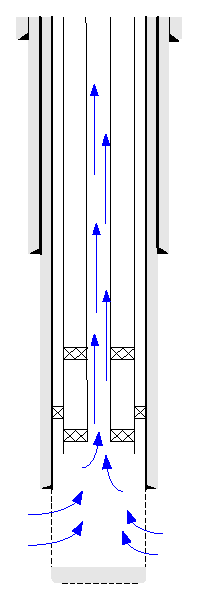
\includegraphics[width=.15\textwidth]{fig/foamer/velocitystring/velocitystring-long.eps}}\label{fig:velocitystring-long}}
    \caption{Schema di applicazione della velocity string \parencite{arachman2004liquid}} 
    \label{fig:velocitystring}
\end{figure}

L'installazione della velocity string è generalmente molto economica rispetto ad altre sistemi di sollevamento artificiale, visto che l'applicazione può avvenire anche tramite \textit{coiled tubing}, prodotti tubolari continui a sezione limitata, fabbricati in lunghezza e avvolti attorno a una bobina di raccolta \parencite{international2014introduction}. Tuttavia la progettazione deve avvenire con particolare cautela, visto che il restringimento della sezione di produzione si traduce non solo in termini di aumento di velocità, ma anche di aumento delle perdite di carico per attrito. La velocity string non è considerata una soluzione definitiva per il GWD, dal momento che il dimensionamento ideale del tubino di produzione ausiliario cambia con l'evoluzione delle condizioni del giacimento.

\subsection{Compressione}
La compressione viene impiegata per diminuire la pressione a testa pozzo. La modalità di compressione può essere a opera di un singolo compressore (\figref{fig:compressore}) o di un sistema di compressori posti in superficie. 

\begin{figure}[htbp]
    \centering
    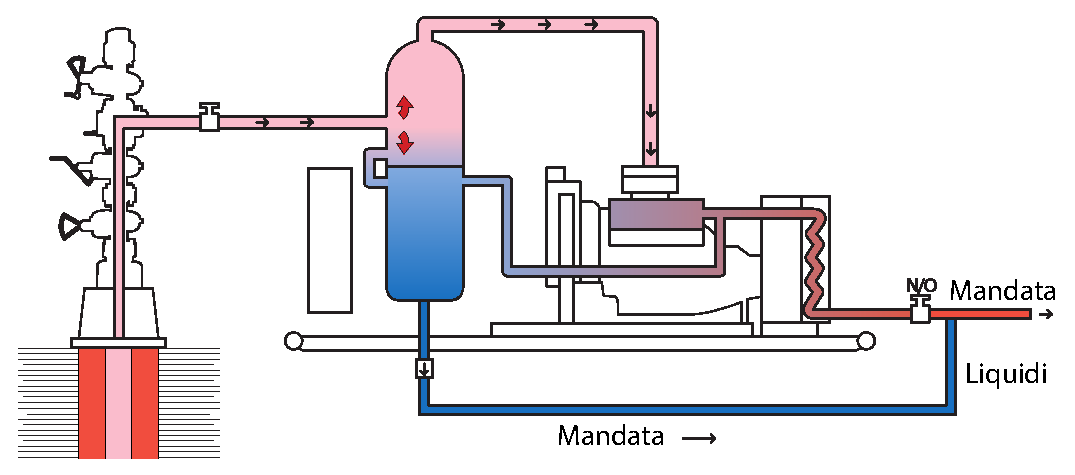
\includegraphics[width=\textwidth]{fig/foamer/compressore.eps}
    \caption{Layout semplificato del GasJack™, copressore singolo utilizzato per operazioni di compressione della testa pozzo \parencite{garner2009backside}}
    \label{fig:compressore}
\end{figure}

Una minore pressione a testa pozzo porta alla diminuzione dell'acqua proveniente da fenomeni di condensazione ma soprattutto all'aumento dell'afflusso di gas in pozzo dal giacimento. L'aumento di portata è associato all'aumento della velocità del gas, raggiungendo così valori al di sopra della velocità critica. Il dimensionamento dell'impianto di compressione si basa sulla pressione di aspirazione e la pressione di mandata, ovvero dal \textit{rapporto di compressione}. \'E importante tenere presente che una minima variazione delle pressioni di aspirazione o di mandata può aumentare in maniera significativa la potenza richiesta dal compressore. La compressione e la riduzione della pressione atesta pozzo sono generalmente le prime soluzioni impiegate per il sollevamento artificiale. L'installazione dei compressori può avvenire durante il ciclo di vita del pozzo senza evidenti segnali di \textit{liquid loading}: la diminuzione di pressione consente di lavorare in condizioni migliori, aumentando le performance generali e quindi la produzione di gas giornaliera. La compressione può anche considerarsi un sistema di sollevamento artificiale ausiliario: un compressore può interfacciarsi con altre soluzioni come agenti surfattanti, gas lift, plunger, beam pump, ESP o velocity string, aumentanto in modo significativo le performance di liquid unloading. La compressione può essere impiegata anche per avviare nuovamente un pozzo morto tramite un kick indotto dal nuovo gradiente di pressione: soluzione alquanto inusuale, l'esperienza sul campo dice che solitamente una diminuzione di pressione non è sufficiente a garantire l'energia necessaria al pozzo per poter spiazzare anche parzialmente la colonna liquida presente.

\subsection{Plunger}

I plunger sono dei dispositivi installati all'interno del pozzo capaci di rimuovere liquidi e altri agenti contaminanti meccanicamente. Il plunger è un pistone tuffante che viaggia liberamente dal fondo pozzo alla superficie, spinto da una pressione che deve essere sufficiente a trascinare sia il dispositivo che i fluidi accumulati. La produzione di gas con l'installazione di un plunger risulta discontinua, legata alla ciclicità del plunger che deve percorre in entrambe le direzioni tutta la lunghezza del pozzo. Come si può vedere nella \figref{fig:conventionalplunger} l'applicazione di un plunger in pozzo richiede l'installazione di determinati impianti di superficie (valvole) e impianti di fondo pozzo (plunger e meccanismo a molla). Una tipica installazione di plunger convenzionale è organizzata nel seguente modo:

\begin{itemize}
    \item \textbf{bumper a molla}, utile a ricevere il plunger a fondo pozzo e evitare danni dovuti all'impatto a terra;
    \item \textbf{ricevitore di superficie}, blocca il plunger una volta giunto in superficie e consente il deflusso del gas in condotta;
    \item \textbf{valvola motorizzata di superficie}, controllata elettronicamente, apre e chiude il pozzo quando necessario;
    \item \textbf{sensore elettronico di superficie}, si attiva quando il plunger giunge in superficie;
    \item \textbf{controller elettronici}, con ciclicità impostata da operatore, gestisce tutte le operazioni di produzione e registra dati in continuo.
\end{itemize}

\begin{figure}[htbp]
    \centering
    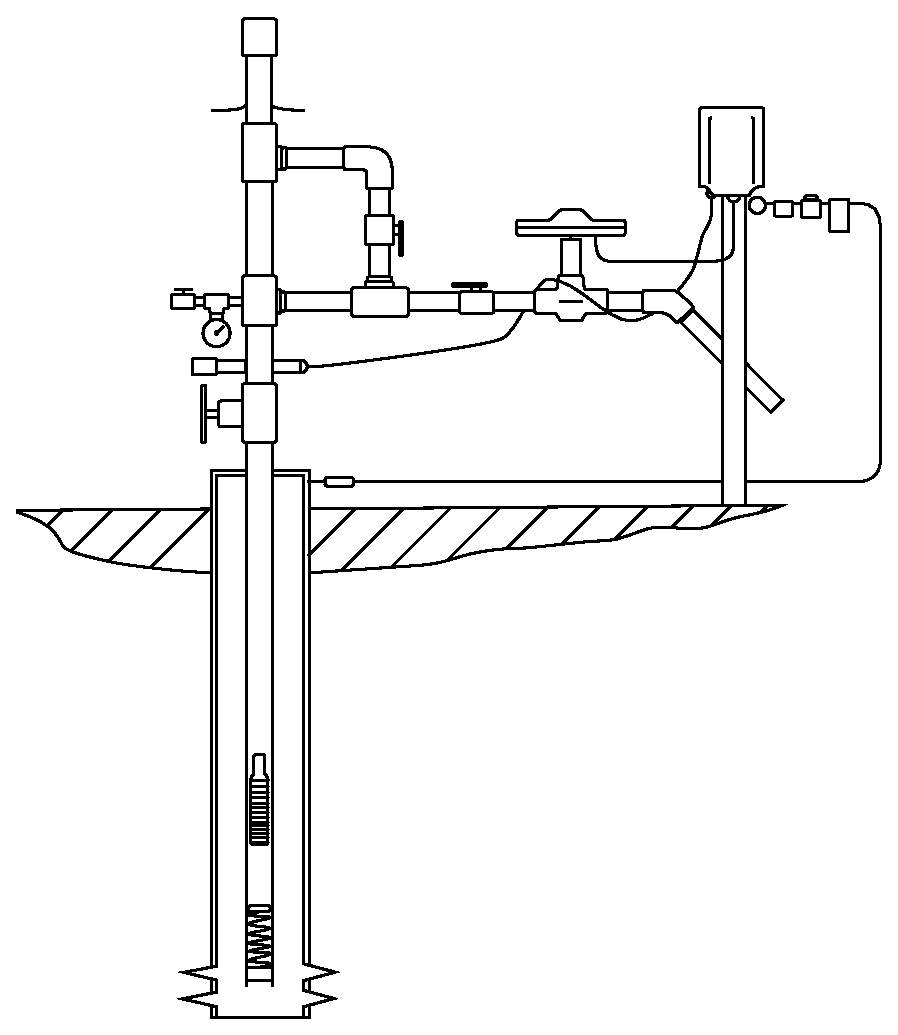
\includegraphics[width=0.6\textwidth]{fig/foamer/plunger-installation.eps}
    \caption{Tipica installazione di plunger \parencite{lea2011gas}}
    \label{fig:plunger-installation}
\end{figure}

Come già detto, l'applicazione di un plunger convenzionale trasforma la produzione da continua a ciclica, caratterizzata quindi da \textit{shut-in} programmati per far tornare il plunger a fondo pozzo e permettere al pozzo, in caso di bisogno, di raggiungere una pressione sufficiente tale da poter trascinare il plunger assieme alla colonna di fluido presente. La \figref{fig:conventionalplunger} mostra un generico ciclo di produzione di un plunger convenzionale:
\begin{enumerate}
    \item[a)] plunger a fondo pozzo con liquido al di sopra, valvola di superficie chiusa;
    \item[b)] apertura della valvola di superficie e risalita del plunger assieme alla colonna liquida;
    \item[c)] fase produttiva del pozzo in assenza di cadute di pressione dovute a liquid loading;
    \item[d)] riaccumulo di fluido a fondo pozzo;
    \item[e)] chiusura del pozzo e discesa del plunger a fondo pozzo.
\end{enumerate}

\begin{figure}[htbp]
    \centering
    \subfloat[][]
    {\centering 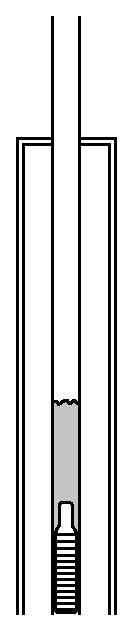
\includegraphics[height=.3\textheight]{fig/foamer/plunger-conventional/conventionalplunger-A.eps}} \label{fig:plunger-conventional-A} \qquad \qquad
    \subfloat[][]
    {\centering 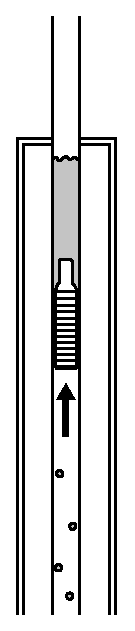
\includegraphics[height=.3\textheight]{fig/foamer/plunger-conventional/conventionalplunger-B.eps} \label{fig:plunger-conventional-B}}  \qquad \qquad
    \subfloat[][]
    {\centering 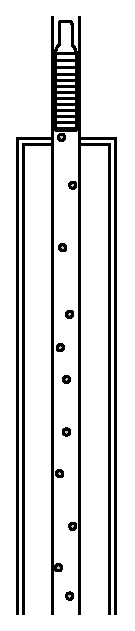
\includegraphics[height=.3\textheight]{fig/foamer/plunger-conventional/conventionalplunger-C.eps} \label{fig:plunger-conventional-C}} \qquad \qquad
    \subfloat[][]
    {\centering 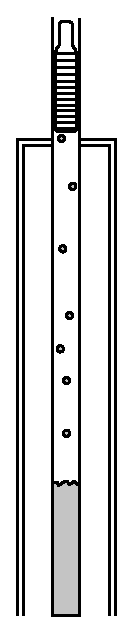
\includegraphics[height=.3\textheight]{fig/foamer/plunger-conventional/conventionalplunger-D.eps} \label{fig:plunger-conventional-D}} \qquad \qquad
    \subfloat[][]
    {\centering 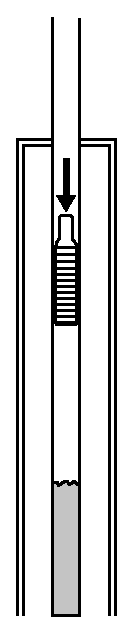
\includegraphics[height=.3\textheight]{fig/foamer/plunger-conventional/conventionalplunger-E.eps} \label{fig:plunger-conventional-E} }
    \caption{Ciclo di un plunger convenzionale}
    \label{fig:conventionalplunger}
\end{figure}

In commercio esistono varie tipologie di plunger e variano a seconda della geometria e degli inserti installati sulla superficie esterna (e.g. spazzole per la pulizia del tubino di produzione). Negli ultimi anni sono nati nuovi sistemi definiti a ciclo libero o in continuo, che permettono la discesa del plunger senza interrompere la produzione. Numerosi sono i brevetti e i prodotti che offrono plunger-lift in continuo: possono essere dotati di una valvola interna (e.g. Weatherford RapidFlo™, FB FreeCycle™ o McClain™) oppure a due pezzi (e.g. Peacemaker™, composto da una sfera e un manicotto). La \figref{fig:plunger} mostra alcune tipologie di plunger presenti sul mercato.\\
L'applicazione di plunger in pozzo per il sollevamento artificiale richiede un investimento iniziale relativamente basso, ma dei costi operativi che possono incidere col tempo e portare a un aumento imprevisto del costo di produzione del gas. Gli investimenti iniziali indiretti possono però incidere fortemente sulla scelta del plunger: la variazione dei volumi di gas e liquido rende necessaria una nuova valutazione circa il dimensionamento degl impianti di trattamento a valle del pozzo, i costi iniziali possono essere quindi legati per esempio all'installazione di un nuovo separatore.

\begin{figure}[htbp]
\centering
    \subfloat[][A spirale]
    {\makebox[0.2\textwidth]{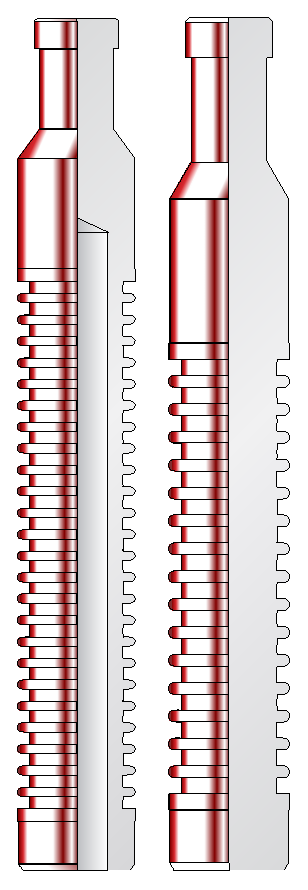
\includegraphics[height=.25\textheight]{fig/foamer/plunger/plunger-spiral.eps}} \label{fig:plunger-spiral}} \quad
    \subfloat[][T-pad]
    {\makebox[0.2\textwidth]{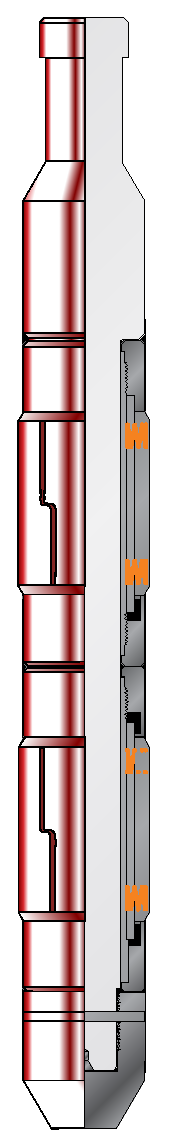
\includegraphics[height=.25\textheight]{fig/foamer/plunger/plunger-tpad.eps}} \label{fig:plunger-tpad}}  \quad
    \subfloat[][A spazzole fisse]
    {\makebox[0.2\textwidth]{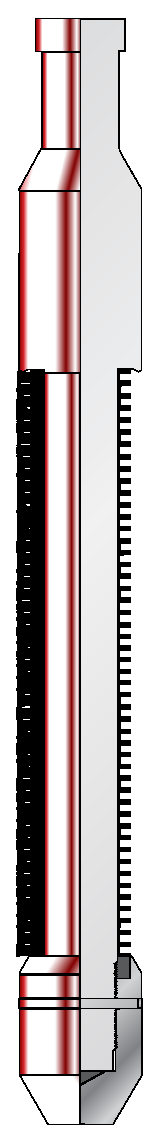
\includegraphics[height=.25\textheight]{fig/foamer/plunger/plunger-fixedbrush.eps}} \label{fig:plunger-fixedbrush}} \quad
    \subfloat[][RapidFlo™]
    {\makebox[0.25\textwidth]{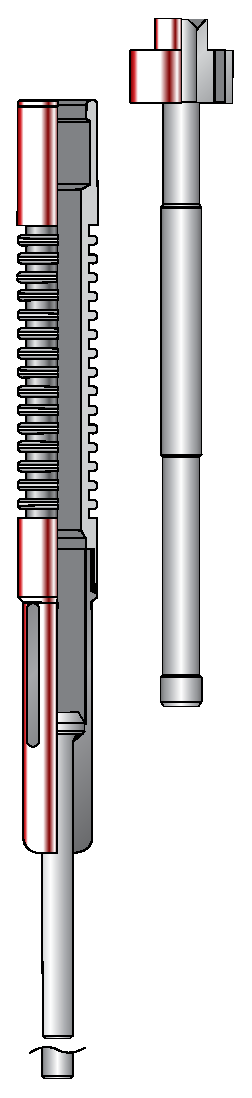
\includegraphics[height=.25\textheight]{fig/foamer/plunger/plunger-rapidflo.eps}} \label{fig:plunger-rapidflo} }
\caption{Principali tipologie di plunger proposte da Weatherford \parencite{weatherford2008brochure}}
\label{fig:plunger}
\end{figure}

\subsection[Altri sistemi per GWD]{Altri sistemi di sollevamento artificiale per deliquification}
Alcune tecnologie per l'attenuazione del battente idrostatico in pozzo nascono da applicazioni pensate in origine per il sollevamento artificiale di giacimenti a olio. Questi sistemi sono stati riadattati per il trascinamento dell'acqua a fondo pozzo o per agevolare l'afflusso del gas in pozzo. I sistemi presentati nel paragrafo corrente sono tutti a energia esterna.
\paragraph{Gas lift}
Il gas lift per dewatering consiste nell'iniezione di gas da una fonte esterna al pozzo a una certa profondità. Nel campo dell'olio il gas iniettato a fondo pozzo diminuisce la densità dell'olio, facilitando così il flusso in condotta. In questo caso viene fatto fluire gas a fondo pozzo sia per diminuire la densità della colonna idrostatica, sia per aumentare la produzione di gas effettiva e quindi l'efficacia di trascinamento della colonna idrostatica da parte della corrente gassosa. Questo sistema gode il vantaggio di non provocare significative variazioni alle conduzioni di produttività  del pozzo e riesce a lavorare anche in perforazioni deviate. L'applicazione purtroppo dipende fortemente dalla presenza di una sorgente di gas ad alta pressione, rappresentata da un pozzo nella zona limitrofe o l'installazione di un compressore, a cui però sono associati alti costi operativi. Per di più il tubino di produzione deve essere progettato per sopportare l'aumento di pressione che si ha in condotta e l'impiego di gas ad alta pressione può portare facilmente a problemi di congelamento e creazione di idrati.
\paragraph{Sistemi di pompaggio}
Le pompe petrolifere o a cavalletto (\textit{Beam Pump} o BP, impiegate in modo massiccio per il sollevamento artificiale per giacimenti a olio, rappresentano il sistema di pompaggio più comune anche nel GWD. Generalmente i sistemi di pompaggio spingono la colonna idrostatica lungo il tubino di produzione (o un tubino ausiliario, come un coiled tubing installato a posteriori) e il gas prodotto viene fatto fluire nell'annulus. Altri sistemi di pompe utilizzate anche in questo campo sono le pompe elettriche sommerse (\textit{Electrical Submersible Pump} o  ESP), pompe a cavità progressiva (\textit{Progressing Cavity Pump} o PCP) e pompe idrauliche (a pistone o \textit{jet pump}). Le pompe vengono generalmente impiegate quando la pressione a fondo pozzo è relativamente bassa e quando il rapporto gas/liquido non è sufficiente da garantire lo spiazzamento della colonna idrostatica tramite i sistemi a energia interna. Le pompe non possono operare in presenza di gas, perciò vanno opportunamente collocate al di sotto degli spari, in modo da ottenere una buona separazione del liquido dal gas. La vita media delle pompe dipende fortemente dagli agenti di erosione, è importante capire se la produzione di liquidi e gas comporta anche la produzione di gas

\section{Schiumogeni}
L'impiego di schiumogeni nell'industria petrolifera è vario e ormai consolidato nel tempo. Come visibile in \tabref{tab:surfactantapplications} i tensioattivi sono impiegati in tutte le fasi di recupero del greggio e nell'industria di processo, dalle perforazioni, iniezioni in giacimento, produzione, al trasporto in condotta onshore e offshore.

\begin{table}[htbp]
    \small
    \centering
    \caption{Alcuni esempi di applicazioni di tensioattivi nell'industria petrolifera \parencite{schramm2006emulsions}}
    \label{tab:surfactantapplications}
\begin{tabular}{p{.8\textwidth}p{.1\textwidth}}
\hline
{\bf Applicazione}                                                         & {\textbf{Fasi}\footnote{Si riferisce alle dispersioni di foamer in fase acqua (\textit{water}, W), fase olio (O), fase gas (G) e fase solida (S)}}           \\ \hline
Fluidi di perforazione con schiume                                         & G/W                    \\
Fluidi di stimolazione e fratturazione con schiume                         & G/W                    \\
Fluidi acidificanti con schiume                                            & G/W                    \\
Recupero di olio freddo e pesante tramite schiume                          & G/O                    \\
Schiume di processo della flottazione dell'olio                            & G/O                    \\
Schiume antincendio                                                        & G/W                    \\
Emulsioni per olio pesante in condotta                                     & O/W                    \\
Emulsioni per la stimolazione pozzo                                        & O/W                    \\
Flottazione di miscele a olio e sabbie bituminose                          & O/W                    \\
Fluidi di perforazione emulsionati (fanghi a base olio)                    & W/O                    \\
Emulsione di catrame e bitumi                                              & O/W                    \\
Emulsioni in situ per EOR                                                  & O/W                    \\
Emulsione di carburanti di trasporto (70\% olio pesante)                   & O/W                    \\
Schiume per il controllo della mobilità del gas                            & G/W                    \\
Sospensioni per fluidi (fanghi) di perforazione                            & S/W                    \\
Sospensioni per fratturazione idraulica e stimolazione del pozzo           & S/W                    \\
Impasti cementizi in pozzo                                                 & S/W                    \\
Solidi di produzione a testa pozzo nel recupero primario dell'olio pesante & S/W                    \\ \hline
\end{tabular}
\end{table}

I tensioattivi sono utilizzati anche in pozzo per mitigare i fenomeni di liquid loading e la tecnica ha ormai acquisito notevole importanza nel GWD. La Nederlandse Aardolie Maatschappij (NAM), compagnia petrolifera olandese, 
ha cominciato a impiegare tensioattivi o \textit{foamer} nei suoi campi a gas nell'ottobre 2003  e dopo soli due anni questo sistema è risultato altamente competitivo rispetto agli altri sistemi per il GWD \parencite{wittfeld2015foam}. 

\subsection{Tensioattivi}
I tensioattivi, surfactanti o agenti attivi di superficie sono composti organici composti al massimo da un gruppo, testa, liofilo e un gruppo, coda, liofobico \figref{fig:sls}. Si parla di testa idrofila e coda idrofoba se il solvente nel quale deve essere utilizzato il tensioattivo è acqua o a base acqua. In termini chimico-fisici la struttura di un surfactante contiene un gruppo polare e da un gruppo apolare.

\begin{figure}[htbp]
    \centering
    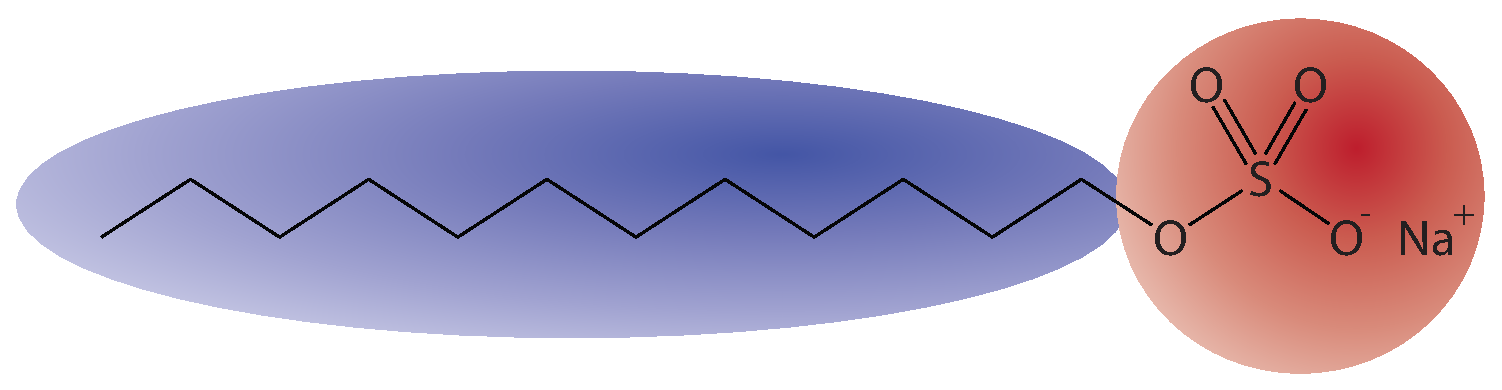
\includegraphics[width=.5\textwidth]{fig/foamer/sls.eps}
    \caption{Laurilsolfato di sodio, tensioattivo anionico utilizzato in molte famiglie di prodotti. La catena a 12 atomi di carbonio rappresenta il gruppo apolare (in blu) mentre il gruppo solfato associato allo ione sodio rappresenta il gruppo polare (in rosso).}
    \label{fig:sls}
\end{figure}

I surfactanti sono classificati in base alla carica del gruppo polare (\figref{fig:surfactants-classification}):
\begin{itemize}
    \item \textbf{anionici}: sali (\ce{Na+}) costituiti da lunghe catene con atomi di carbonio che terminano con un gruppo carbossilato (\ce{COO-})  o solfonato (\ce{SO3-}, \ce{SO4-});
    \item \textbf{cationici}: sali (\ce{Cl-}, \ce{Br-}) di cui è importante la parte positiva, costituita da lunghe catene di atomi di carbonio terminanti con un gruppo ammonico;
    \item \textbf{non ionici}: alcoli a lunga catena, come i derivati poliossietilenici degli acidi grassi;
    \item \textbf{anfoteri} o \textbf{zwitterionici}: tensioattivi anionici in ambiente alcalino, tensiattivi cationici in ambiente acido.
\end{itemize}

\begin{figure}[htbp]
    \centering
    \subfloat[][Anionici]
    {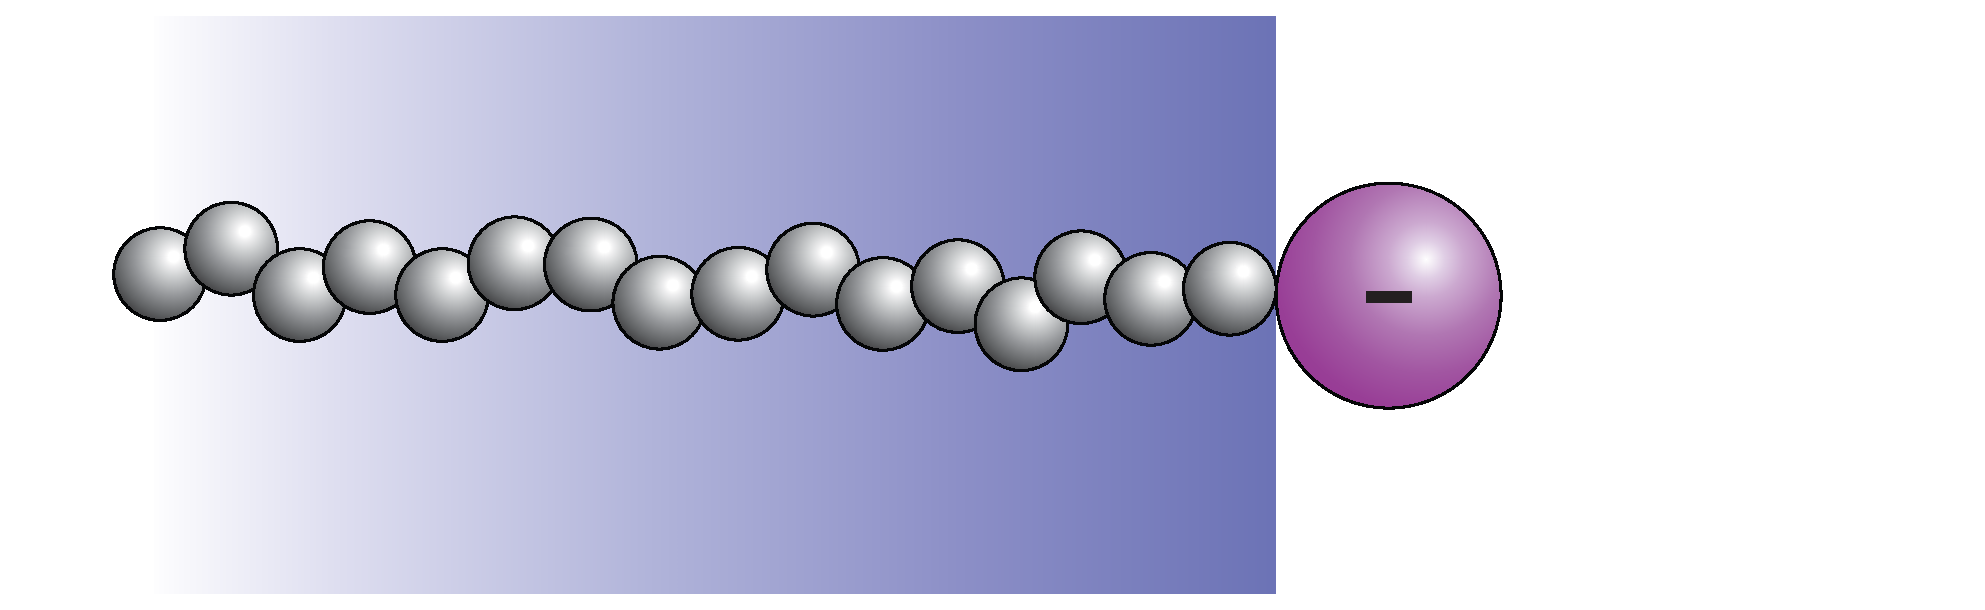
\includegraphics[width=.45\textwidth]{fig/foamer/surfactants-classification/anionic.eps} \label{fig:anionic}} \quad
    \subfloat[][Cationici]
    {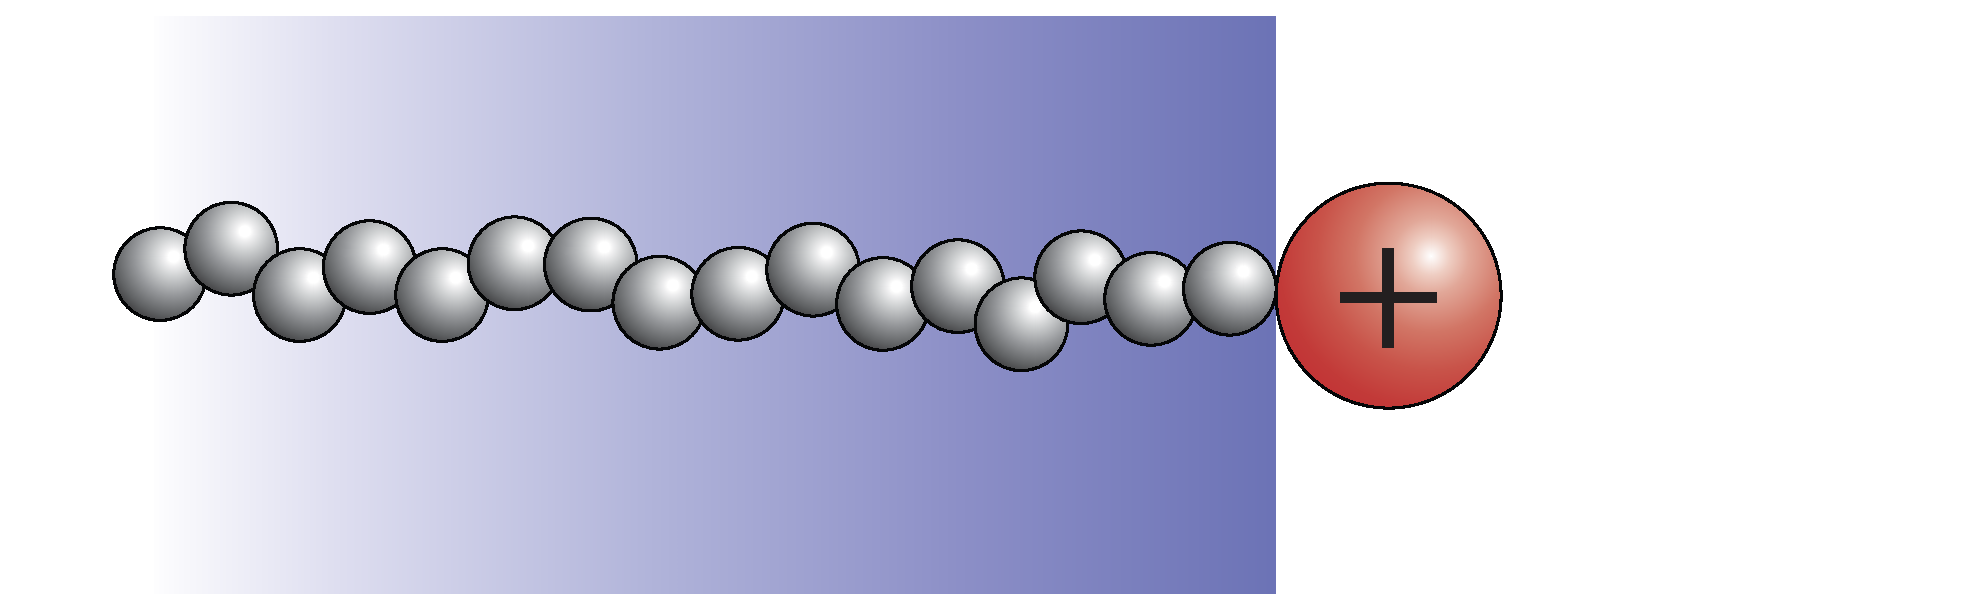
\includegraphics[width=.45\textwidth]{fig/foamer/surfactants-classification/cationic.eps} \label{fig:cationic}}  \\
    \subfloat[][Anfoterici]
    {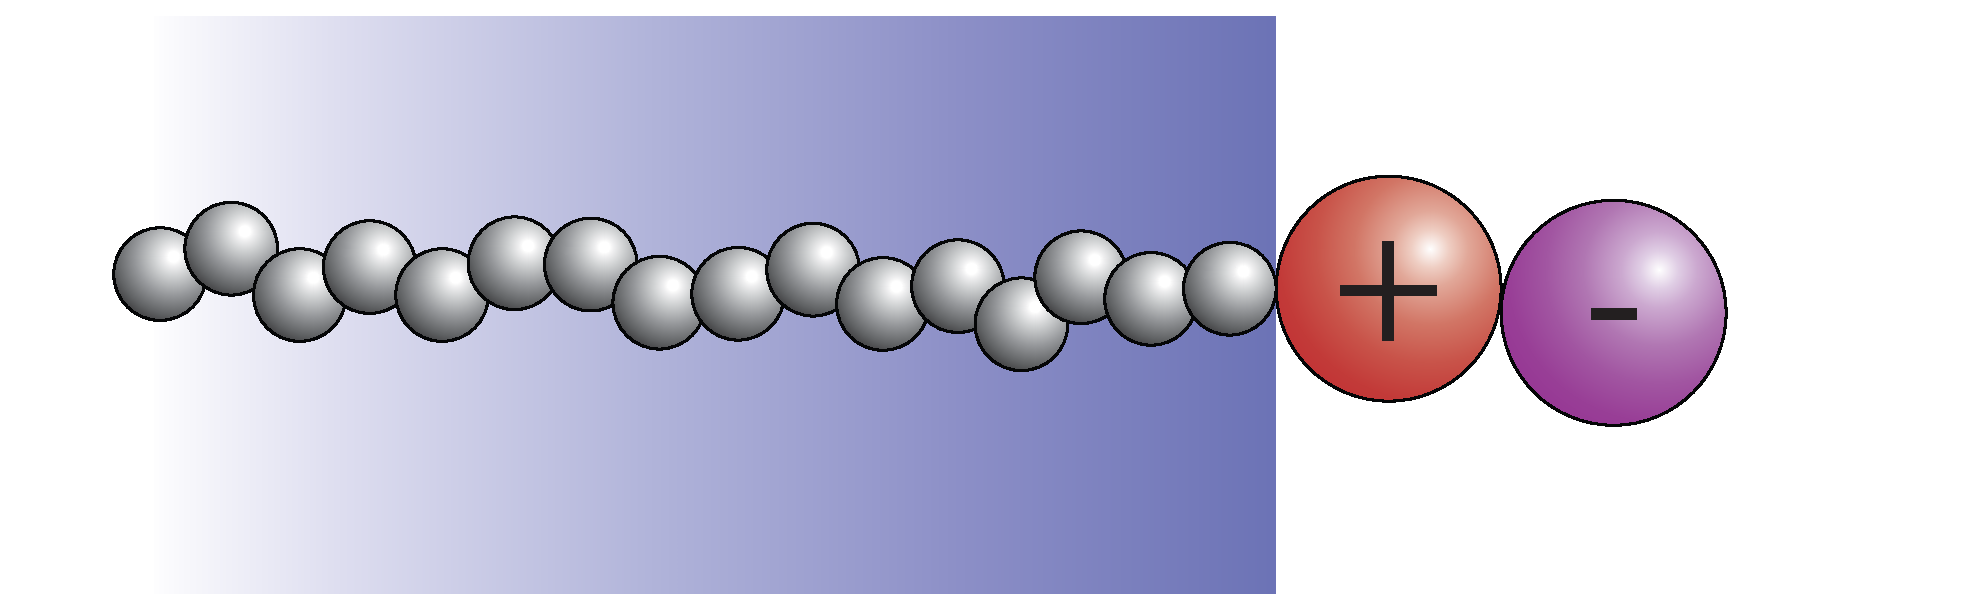
\includegraphics[width=.45\textwidth]{fig/foamer/surfactants-classification/anphoteric.eps} \label{fig:anphoteric}}  \quad
    \subfloat[][Non ionici]
    {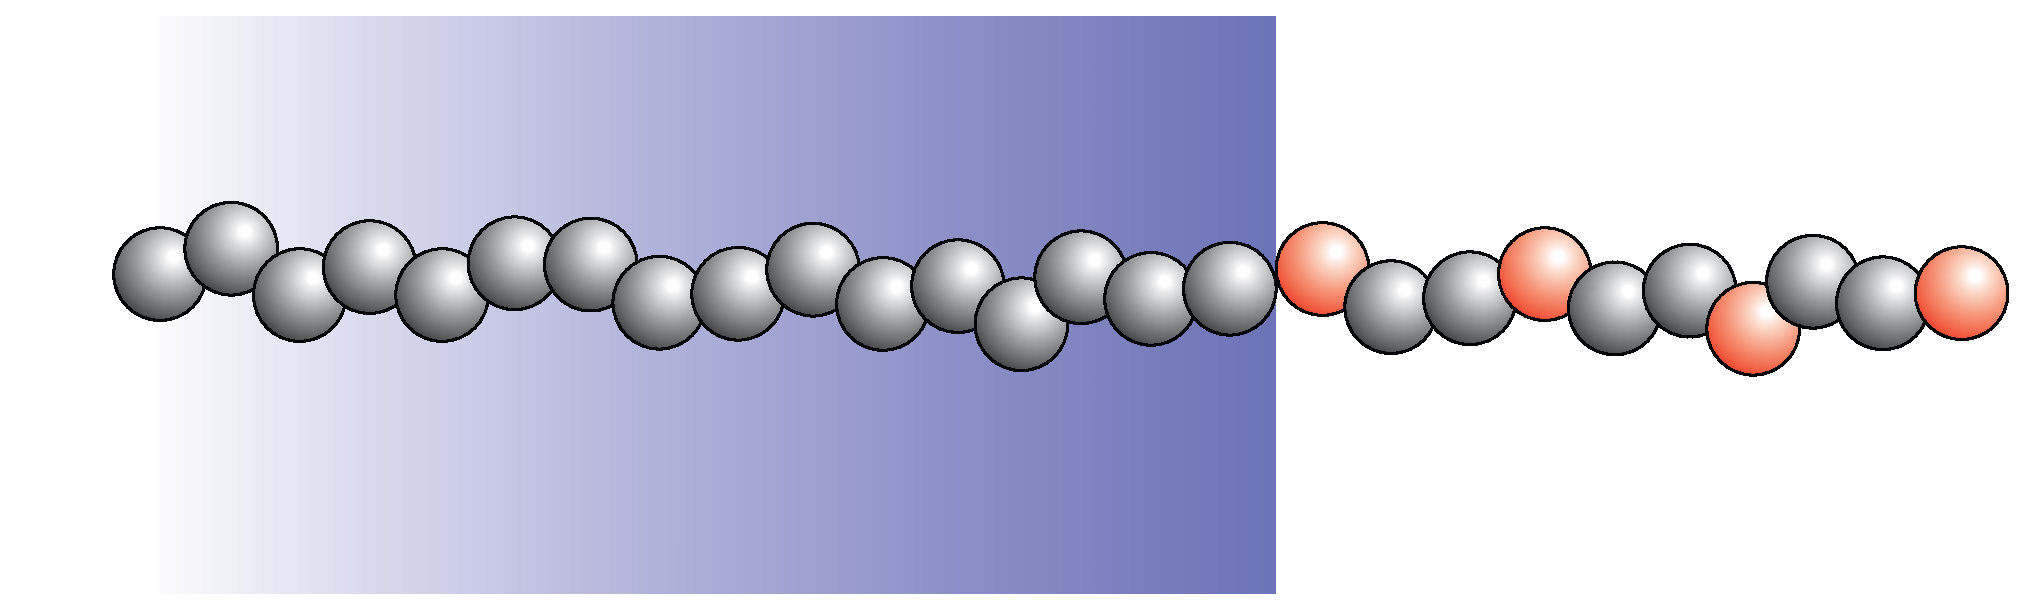
\includegraphics[width=.45\textwidth]{fig/foamer/surfactants-classification/nonionic.eps} \label{fig:nonionic}} 
\caption{Classificazione dei tensioattivi in base alla carica del gruppo polare}
\label{fig:surfactants-classification}
\end{figure}

Due fenomeni derivano dalla presenza di un gruppo polare e apolare all'interno della stessa molecola: adsorbimento e aggregazione.\\
Si consideri un volume d'acqua a contatto con aria dove vengono disciolti dei tensioattivi. I surfactanti, in prossimità della superficie di contatto delle due fasi, si orientano in modo tale che il gruppo polare sia adsorbito dalla fase liquida e il gruppo apolare permanga nella fase gassosa. Tale adsorbimento porta alla diminuzione dell'energia libera di Gibbs o entalpia libera, quindi alla riduzione della tensione superficiali tra le due fasi.. Allo stesso modo i tensioattivi possono diminuire la tensione superficiale di acqua a contatto con una generica fase olio o di un solido, aumentando in questo caso la bagnabilità di quest'ultimo.

Un altro modo per limitare il contatto del gruppo apolare con l'acqua è la creazione di strutture bi- o tridimensionali, capaci di racchiudere i gruppi apolari internamente e mettendo a contatto con l'acqua i gruppi polari \figref{fig:micelle}. Queste strutture sono definite micelle, sono il frutto dei fenomeni di aggregazione dei tensioattivi e possono avere forma lamellare (in questo caso i surfactanti sono molecole anfifiliche o anfifobiche, sferica o cilindrica.  Tali aggregati supramolecolari tendono a crearsi una volta superato un certo valore di concentrazione del surfactante in soluzione, definito \textit{concentrazione micellare minima}. La complessità di tali strutture dipende dalla concentrazione in acqua e dalla specie chimica dell'agente attivo di superficie.

\begin{figure}[htbp]
    \centering
    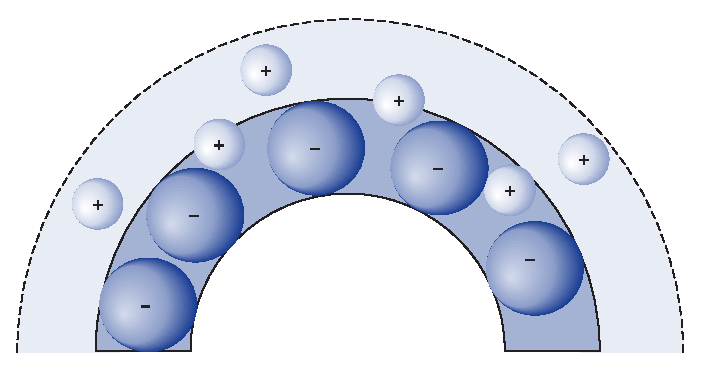
\includegraphics[width=.5\textwidth]{fig/foamer/micelle.eps}
    \caption{Sezione parziale di una micella anionica, il layer compatto negativo generato dall'orientamento del gruppo polare del tensioattivo è circondato dalla fase acqua  \parencite{attwood2012fasttrack}.}
    \label{fig:micelle}
\end{figure}



\section{Applicazioni di schiumogeni per l'attenuazione del liquid loading}
aerhheraeherh

\subsection{Schiumogeni in pozzo}
sdgrahthr
\subsection{Stick}
rtssrtjtysr
\subsubsection{Schiuma in-batch}
srtujrt
\subsubsection{Schiuma in continuo}
rtsustyuy

\section{Confronto tra le tecnologie di sollevamento artificiale per pozzi a gas}
Citare tutti i lavori di GDW 2014-2015